\section{Data Analysis of De-Noising data with AI assistance}

The two data samples, background merged and de-noised, were also processed with new 
reconstruction software, which includes AI assisted track candidate identification~\cite{Gavalian:2022mlp}. The reconstruction software is designed to be able to process data in two parallel branches, where in one branch it reconstructs tracks with conventional algorithm where track candidates are identified by fitting all combinations of clusters forming a candidate and choosing candidates that pass the ``goodness'' of the fit criteria,  and on the second branch AI classifies track from the list of candidates crated from all combinations of clusters forming a track. This procedure is described in detail in~\cite{Gavalian:2022mlp}. Two samples were processed and comparison was made 
between conventional tacking algorithm from raw background merged files, and output of de-noised data sample with and without AI assisted tracking. 

\subsection{Luminosity dependence}

The track reconstruction efficiency was calculated for three samples using Eq.~\ref{eq::eff} for all three reconstructed data samples. The results are presented on Figure~\ref{lscan::conv_dn_ai}. It can be seen from the figure that using AI assisted tracking on de-noised data sample further improves reconstruction efficiency. The raw background merged data sample exhibits tracking efficiency decline of $0.23\%$ per nA, while the combination of de-noising and AI assisted tracking reduces this slope to $0.12\%$ (almost factor of 2), resulting in efficiency of $0.86\%$ at beam current $150~nA$ compared to $0.88\%$ at $45~nA$ beam current. 

\begin{figure}[!h]
\begin{center}
 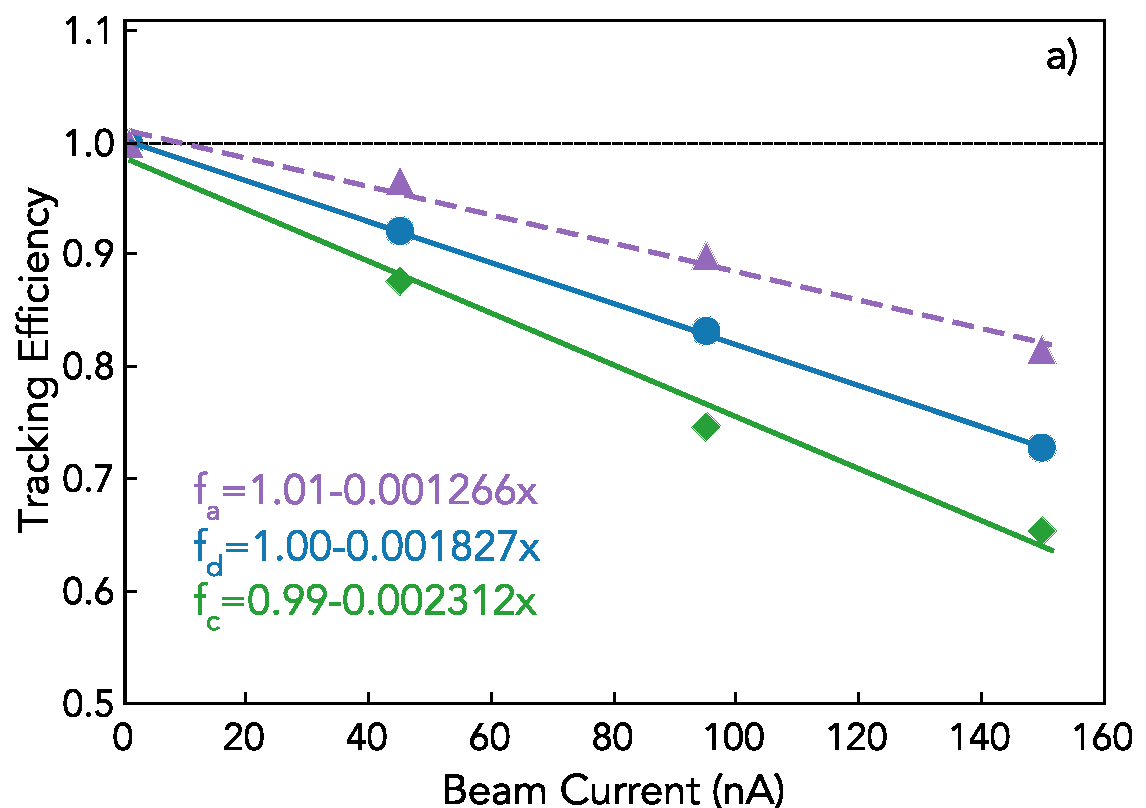
\includegraphics[width=3.1in]{images/figure_lscan_pos_ai.pdf}
 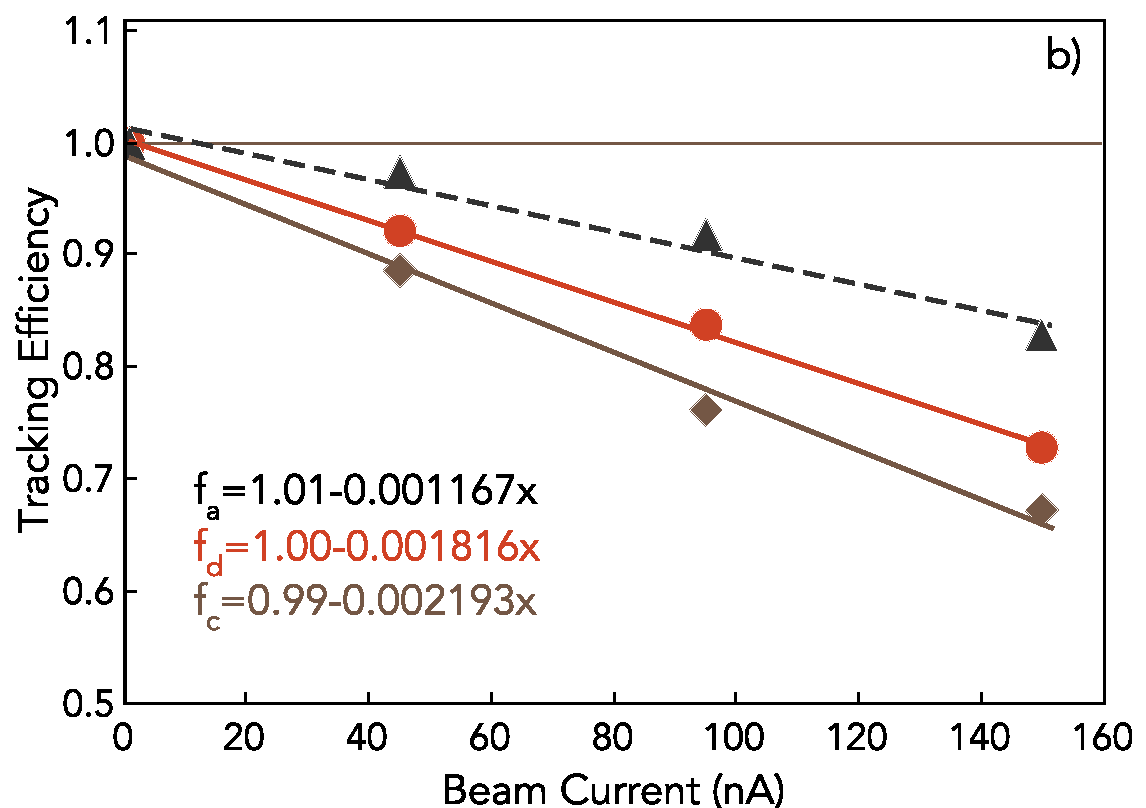
\includegraphics[width=3in]{images/figure_lscan_neg_ai.pdf}
\caption {Tracking efficiency as a function of luminosity (beam current) for positive (a) and negative particle (b).  The efficiency is shown for
conventional algorithm running on background merged files (diamonds), and on files with merged background then de-noised with AI (circles).}
 \label{lscan::conv_dn_ai}
 \end{center}
\end{figure}

This is significant improvement in tracking efficiency when using both AI assisted tracking with de-noising for beam current 3 times higher than current data collecting conditions.

\subsection{Physics Impact}

Further the physics impact was studied for de-noised data sample processed with AI assisted tracking. Same data sample was used in this studies with selected $H(e,e^-\pi^+\pi^-p)X$ event from Pythia simulations, and analyzed for
missing mass of $H(e,e^-\pi^+\pi^-)X$. The distributions of missing mass spectra are shown on Figure~\ref{physics::conv_dn_ai}.

\begin{figure}[!h]
\begin{center}
 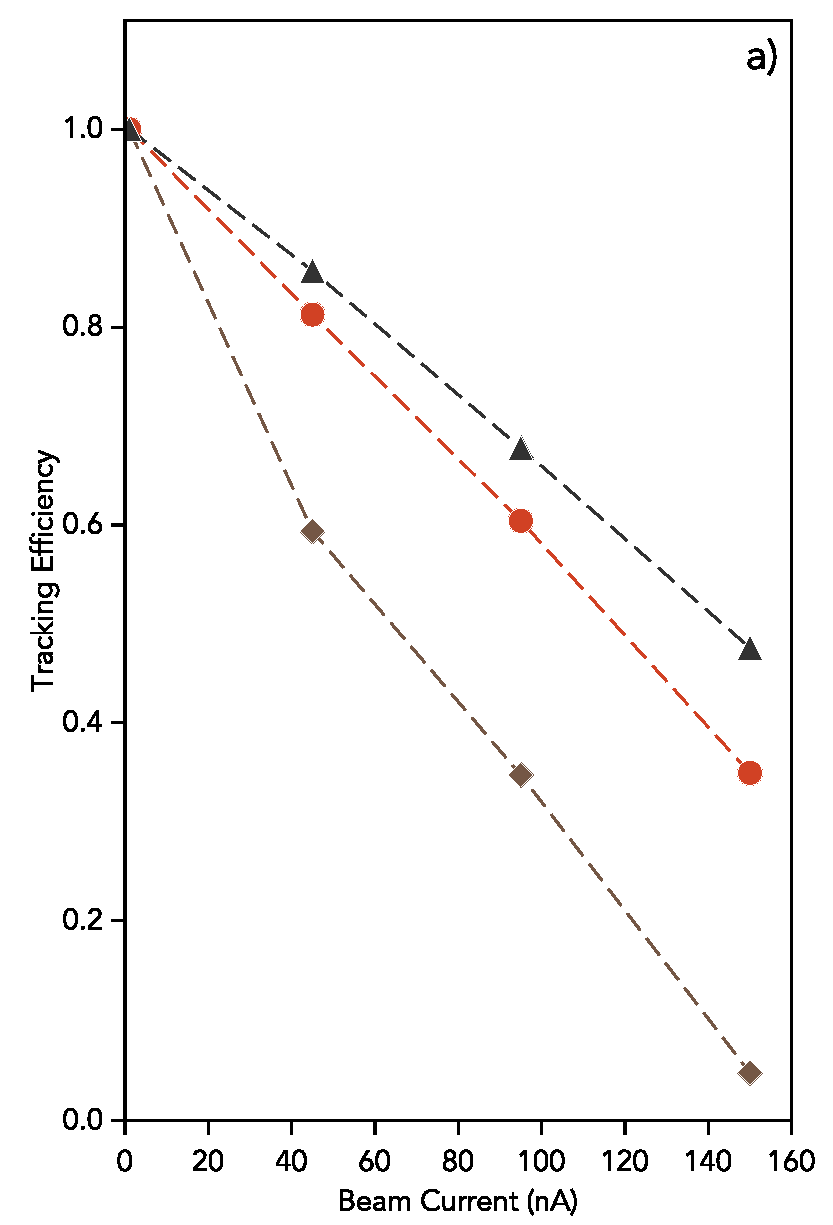
\includegraphics[height=3.0in]{images/figure_phys_scan_ai.pdf}
 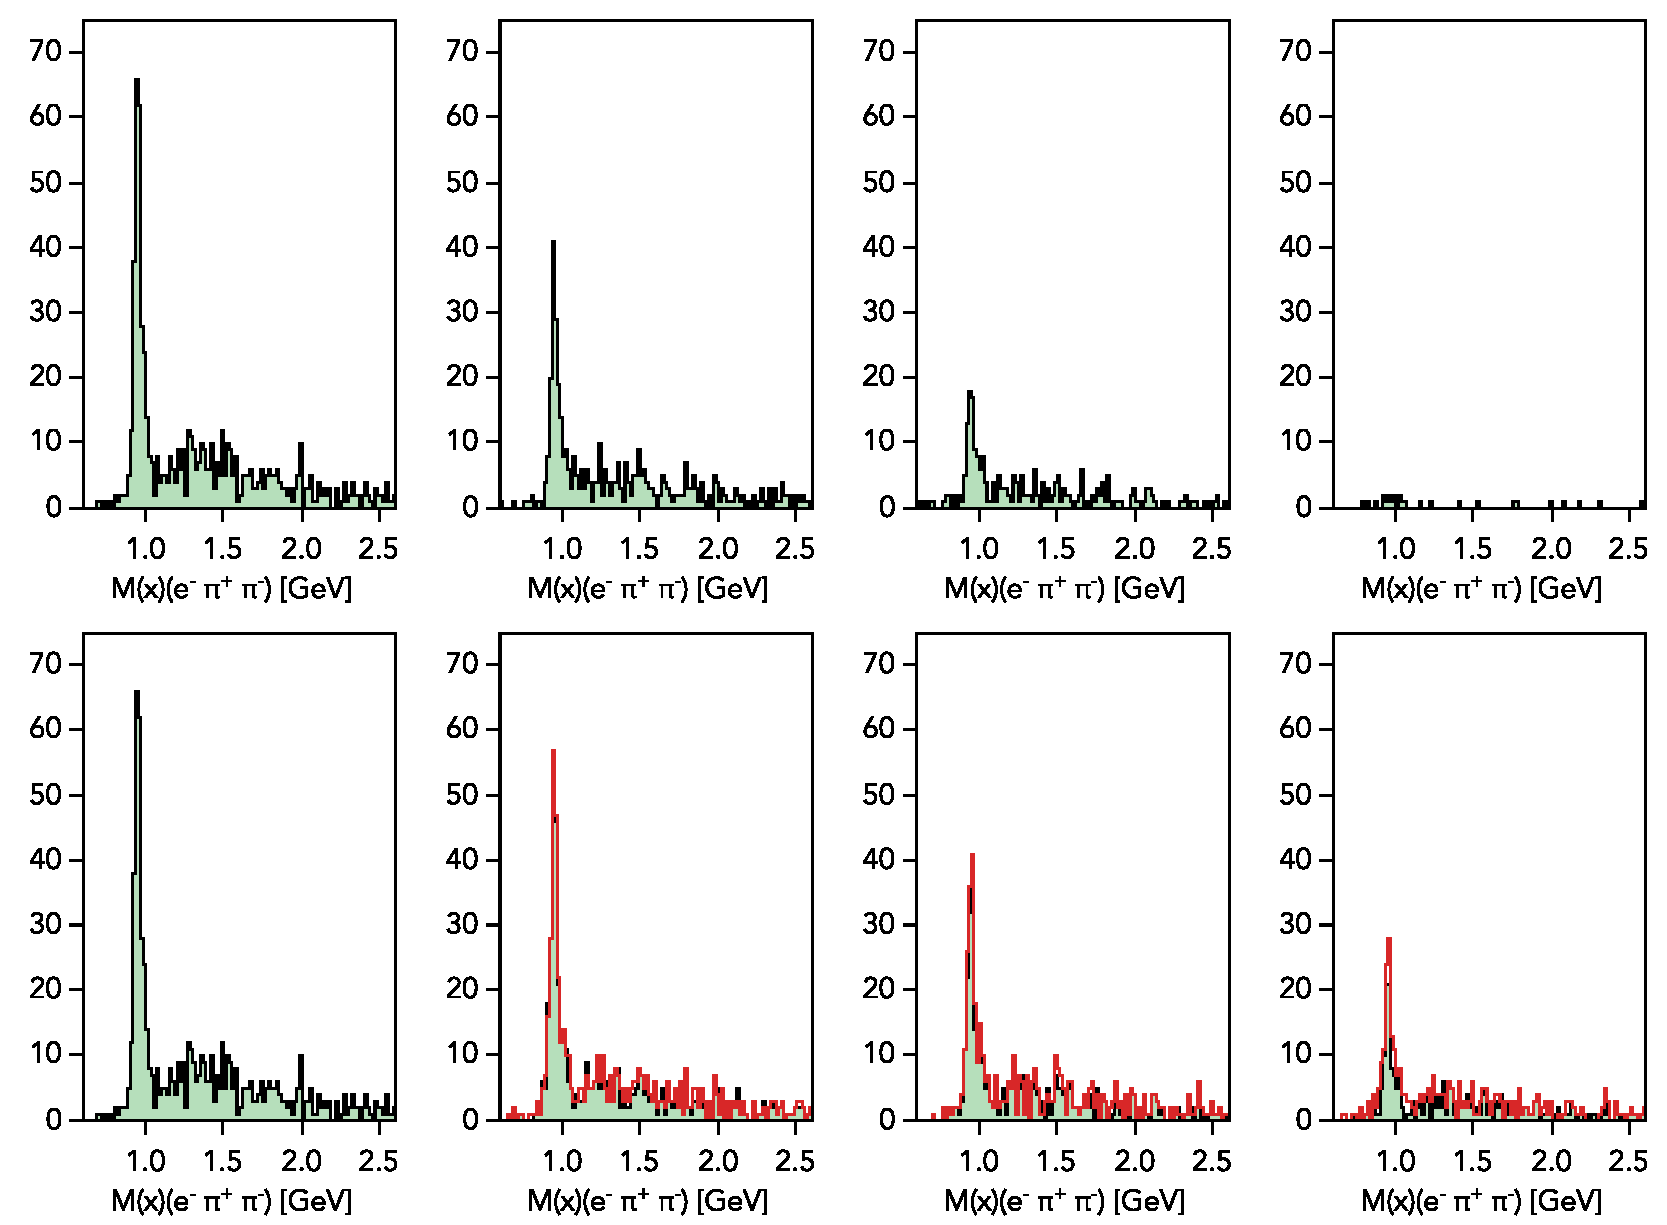
\includegraphics[height=3.0in]{images/figure_phys_conv_ai.pdf}
\caption {Number of reconstructed protons from missing mass of $H(e \rightarrow e^\prime \pi^+\pi^-)$ for background 
merged files for  $5~nA$, $45~nA$, $95~nA$ and $150~nA$ respectively. The number of protons reconstructed by 
conventional algorithm after background merging is shown on the top row, and reconstruction after  de-noising drift 
chamber data on the bottom row.}
 \label{physics::conv_dn_ai}
 \end{center}
\end{figure}

The top row of plots shows missing mass distributions for different backgrounds reconstructed by conventional tracking algorithm. On the bottom row the distributions reconstructed from de-noised data sample are shown, with overlaid histograms (red) of AI assisted reconstruction. On Figure~\ref{physics::conv_dn_ai} a) the summarized analysis of missing mass distributions are shown where number of reconstructed protons are plotted for all three reconstruction scenarios. It is evident that adding AI assistance for track classification further improves physics outcome from data processing. It can be seen that for $95~nA$ data sample, the number of reconstructed protons with de-noising and AI assisted tracking is $14\%$ higher than number of protons from background merged file reconstructed using conventional (no AI involved) code.




